% DOCX paragraph 192
\chapter{Spacetime, Curvature and Gravity}\label{ch:03}

% DOCX paragraph 193
% Title continued in paragraph 192.

% DOCX paragraph 196
This chapter has the daring ambition of explaining a series of abstract concepts
underlying Einstein's theory of general relativity\index{general relativity} in a simple way.
The mathematics of this theory can express such concepts in a transparent and elegant
manner, and, for a physicist or a mathematician, (almost) everything is clear as soon as
the corresponding equations are written down. So, I could simply show them and say,
``It's all there, don't you see?''. I know, however, that such an approach would not
take us very far, while my commitment is to be your vigilant guide on this journey.

% DOCX paragraph 197
So, what I am going to do is definitely more difficult: to illustrate this new
interpretation of gravity using concepts we are all used to. The challenge in this
approach is not so much related to the complexity of the concepts (which is all in the
mathematics) but with the effort necessary to accept an interpretation of physical
reality that is often in contrast to our everyday experience. In other words, what I am
asking is that you imagine a reality that can be very far from what you are used to. But
on the other hand, imagination is one of the requirements of this journey.

% DOCX paragraph 198
So let us start from where the previous chapter ended, namely, when we said that the
Einstein equations elegantly summarise the equivalence between gravity and the
curvature\index{curvature} of spacetime. To be more precise, we wrote that these
equations essentially state that:

% DOCX paragraph 200
\begin{equation}\label{eq:03-01}
\begin{pmatrix}
gravity\ is\ the\ manifestation\ of\  \\
spacetime\ curvature
\end{pmatrix}
\end{equation}

% DOCX paragraph 201
% Equation number is generated with the preceding equation.

% DOCX paragraph 203
I know from experience --- and from reading the faces of far too many students when
first written on a blackboard --- that this sentence sounds fundamentally obscure.
However, it is correct and absolutely true, at least in so far as we can verify it
through scientific experiments. Do not despair, though, and, above all, do not give up
now! Later on, when we return to this statement, you will find yourself able to
understand it and even appreciate its profound implications.

% DOCX paragraph 206
\section[Spacetime]{Spacetime: Everything That Has Happened and Will Happen}\label{sec:03-spacetime}

% DOCX paragraph 208
To understand what Equation \eqref{eq:03-01} actually states, we can analyse the various terms that
it contains. So, let us start from the concept of \emph{spacetime}. First of all, it
should be noted that I have not written ``space-and-time'', nor ``space-time'', but
``spacetime''. It may seem a minimal, irrelevant difference, but it is instead
fundamental because it represents one of the first lessons of the theory of general
relativity. This is because Einstein postulates that our idea of space and time as
distinct entities is incorrect since the two are completely equivalent. It follows that
a shift in space from one point to another is equivalent, at the level of the equations,
to a shift in time from one moment to another. Going left or right, up or down, is not
in any way different, at least mathematically, from going back and forth in time.

% DOCX paragraph 209
In Einstein's theory, therefore, spacetime is a single object, which can be seen in
essence as a ``container'' of elements (i.e., termed a ``set'' in mathematics) that are
also referred to as \emph{events}. Let me explain by offering an example: The European
Union can be considered a ``set'' of citizens from its various countries; such citizens
are therefore the building blocks, or elements, of the European Union. Similarly,
spacetime is the set of all events: past, present, and future. An
event\index{event (spacetime)} (an element of spacetime) is understood to be something that
has happened, is happening or will happen somewhere at some time. The alarm clock you
set this morning, having breakfast, taking a bus to work~\ldots{} all of these are
events. Reading this book right now is also an event, as it is possible to establish
that it happens in a specific place (for example, on your sofa) and at a specific time
(now). Since each event needs the specification of four different pieces of information
--- three for the position in space and one for that in time --- it is quite simple to
conclude that spacetime is a container in four dimensions (three spatial and one
temporal) of elements called events.

% DOCX paragraph 210
To this definition, Einstein adds that this container of events is not particularly
useful when taken alone and without further rules. Therefore, it is necessary to
associate precise rules to identify the relative position of the various elements, i.e.,
their \emph{distance}. In other words, when considering two events A and B, it is
essential to establish in what relation they are to each other, namely, whether A
occurred before or after B, whether it is to its right or its left, above or below, and
finally, whether the two are somehow connected or, conversely, completely independent.

% DOCX paragraph 211
These rules can only be established by making a choice of
coordinates\index{coordinates}, that is, after introducing an ordered series of numbers
that establish the sequence of events and thus allow us to know the relative position of
A and B. This choice of coordinates is totally arbitrary --- hence the adjective
\emph{relativity} in Einstein's theory --- but the relations among the events that
follow from the selection of coordinates is the same, regardless of the choice made.
This is why, within the theory of general relativity, it is still possible to establish
without ambiguity what you did first this morning: wake up or have
breakfast.\textsuperscript{\hyperlink{note:03-01}{1}} Furthermore, the sequence of events will be the same for
every observer, whatever their state of motion.

% DOCX paragraph 214
\section{Curvature}\label{sec:03-curvature}

% DOCX paragraph 216
Now that we understand what spacetime is, let us go back to our statement \eqref{eq:03-01} and
focus on the second concept that appears there, that of
\emph{curvature}\index{curvature}.

% DOCX paragraph 217
Again, mathematics offers us sophisticated and elegant tools for measuring the curvature
of a surface in a space of arbitrary dimensions. Without going into detail, what we need
to know here is that there are surfaces that can be considered ``curved'' and that their
degree of curvature can be measured using rather simple mathematical tools, one of which
is the concept of \emph{parallel transport}\index{parallel transport} \emph{in a closed
circuit}. The way it works is as follows: take a vector\index{vector} (i.e., an
``arrow'' of a certain length) in a certain portion of spacetime and move it along a
closed loop, making sure it always points in the same direction. If you do this, you are
performing a \emph{parallel}\index{curvature!parallel transport} \emph{transport}, and there is a
mathematical object (called the \emph{Riemann} or \emph{curvature}\index{curvature!tensor (Riemann)}
\emph{tensor}\index{tensor!Riemann}\index{tensor!curvature}) that will measure the amount of
curvature present when going around the loop.

% DOCX paragraph 218
This may sound abstract, but a couple of examples can help clarify this concept.
Therefore, consider a surface in two dimensions, starting from the simplest possible,
that is, a plane. Next, imagine representing the closed circuit by means of a triangle
ABC and using, as a reference for a certain direction, an arrow of a given length whose
origin coincides with point A and whose direction is aligned along the side AB. In
mathematics and physics, an arrow of this type is called a ``vector''
\index{vector} and is characterised by a length and a direction indicated by the
tip of the arrow. We can now slide our vector along AB, bring it to point B, and move it
towards point C. In doing so, however, it is important to keep the initial direction of
the arrow fixed since this is the idea behind parallel transport. Once at C, we will
transport the vector to the AC side and close the circuit, as shown in Figure \ref{fig:03-01}.

% DOCX paragraph 221
\begin{figure}[htbp]
\centering
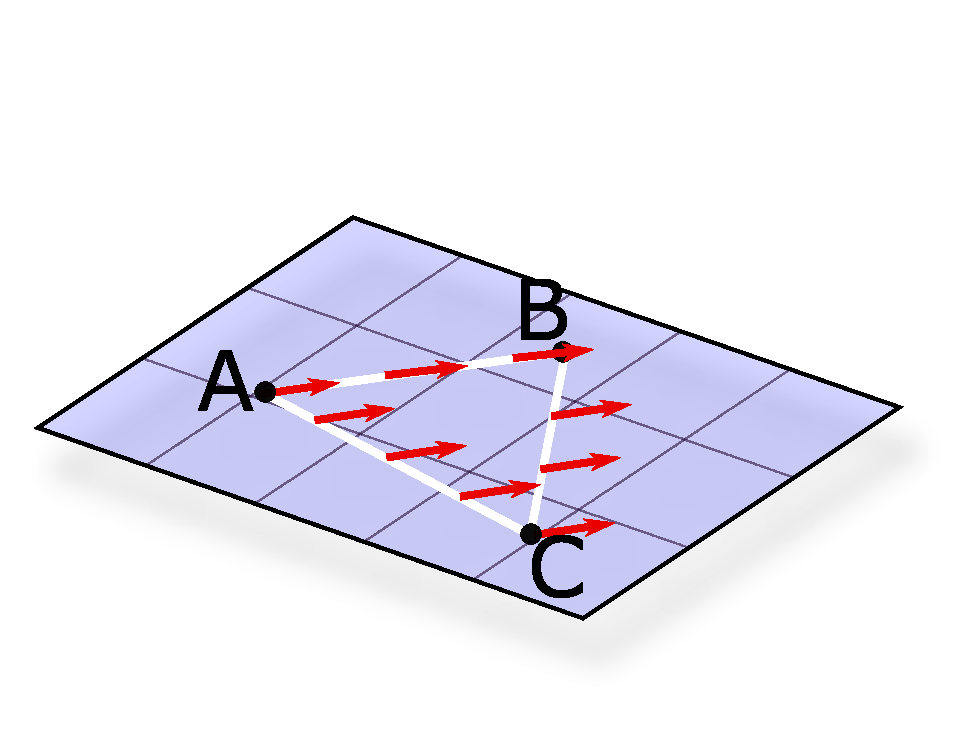
\includegraphics[width=0.88\linewidth,height=0.48\textheight,keepaspectratio]{../figs/pdf/en/fig-03-01.pdf}

% DOCX paragraph 222
\caption{\emph{Parallel transport of an arrow (vector) along the triangle ABC on a
two-dimensional plane. The comparison between the final vector and the initial one at A
shows us that they are identical: the plane is a flat surface because it has zero
curvature.}}\label{fig:03-01}
\end{figure}

% DOCX paragraph 223
At this point, we can compare the final vector\index{vector} with the initial one,
concluding that they are identical: nothing has changed in carrying it in parallel along
a closed loop contained in a plane. Furthermore, we will say that this absence of a
change in the two vectors is linked to the absence of curvature on the surface, that is,
that the plane is a \emph{flat}\index{spacetime!flat} surface because it has zero
curvature\index{curvature!zero (flat)}.

% DOCX paragraph 224
What we need next is an example of a non-flat surface. Let us consider a two-dimensional
surface that mathematicians adore for its simplicity and for the richness of its
properties: a \emph{two-sphere}\index{two-sphere}, that is, the surface of a sphere
with a constant radius. We can think of a two-sphere as the peel of an orange if it were
smooth and very thin, or as a simplified representation of the surface of the Earth.

% DOCX paragraph 225
In this case, we could build our closed circuit (again represented by a triangle ABC) by
connecting two meridians (lines of longitude) through the section of a parallel (line of
latitude) that intersects them. So let us imagine starting from point A, perhaps a
beautiful island in the Caribbean, and pointing north with the help of a compass. As
long as we move precisely following the needle, we are essentially carrying our
vector\index{vector} parallel along the meridian and can therefore reach the North
Pole, that is, point B. There, being careful not to turn around, and thus always looking
in the same direction, we go south following another meridian, for example, the one
placed at a right angle to the first, and we thus reach point C somewhere in northern
Africa. Once we arrive at our destination, at the latitude of A, we move west along the
parallel that forms the side CA of the triangle but always looking in the direction in
which we reach the North Pole.

% DOCX paragraph 226
Once we are back at A and have closed the circuit, as shown in Figure \ref{fig:03-02}, we can
compare the final vector\index{vector} with the initial one, concluding that this
time they are not identical at all: they point in perpendicular directions, the first to
the north and the second to the east!

% DOCX paragraph 228
\begin{figure}[htbp]
\centering
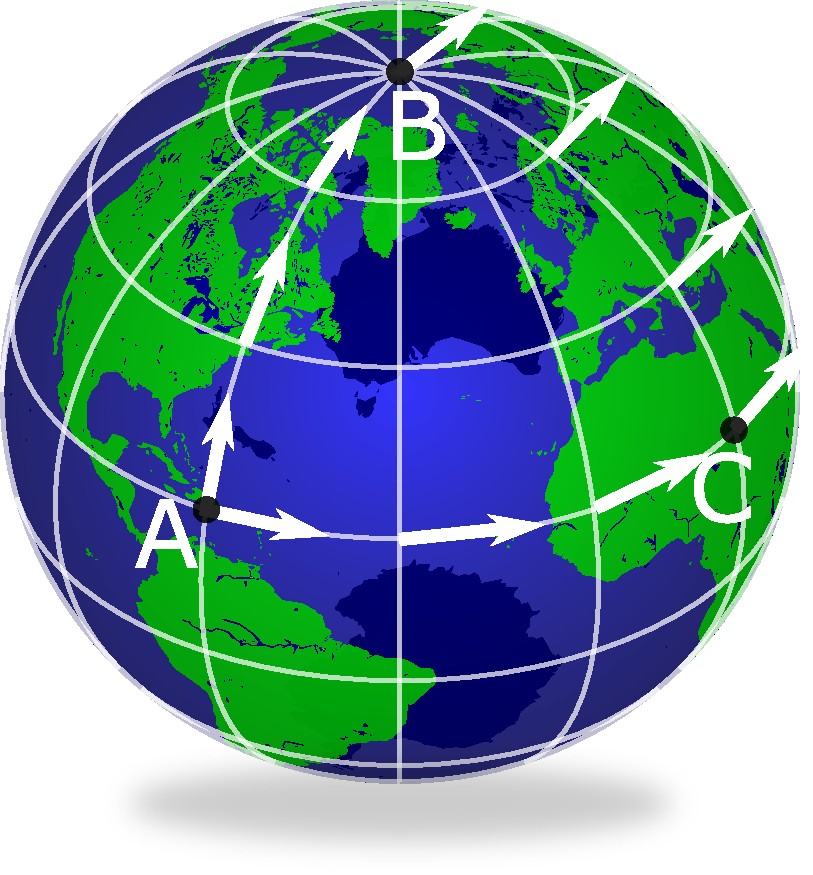
\includegraphics[width=0.88\linewidth,height=0.48\textheight,keepaspectratio]{../figs/pdf/en/fig-03-02.pdf}

% DOCX paragraph 229
\caption{\emph{Parallel transport of a vector along a closed circuit on a
two-sphere}\index{two-sphere}\emph{. The comparison between the final vector and the
initial one shows that the two are different because they point in perpendicular
directions: the two-sphere is a curved surface as it has a non-zero curvature.}}\label{fig:03-02}
\end{figure}

% DOCX paragraph 230
In this way, we have found that the parallel transport\index{parallel transport} of a vector
along a closed loop on a two-sphere\index{two-sphere} introduces a change in the
direction of a vector\index{vector} and that this change is related to the
presence of a curvature on the spherical surface. In other words, we have learned that a
two-sphere is a \emph{curved} surface \index{spacetime!curved}because it has a non-zero
curvature\index{curvature!non-zero (curved)}.

% DOCX paragraph 231
Of course, this simple experiment should be enough to convince flat-earthers of how
foolish their theory is. But it also reveals something very interesting and invites us
to a series of important reflections. The first is that if we had chosen a very small
triangle, the variation between the two vectors would have been less evident. For
example, if we considered a triangle with sides of just a hundred metres, it would have
been very difficult to measure the difference between the vectors without very
sophisticated tools. Therefore, a curved surface can be approximated, at least
\emph{locally} (i.e., in the vicinity of each of its points), with a
flat\index{spacetime!flat (locally)} surface. In other words, the effects of curvature are evident
only on scales comparable to the so-called \emph{curvature radius}\index{spacetime!curvature radius}
of the curved surface.

% DOCX paragraph 232
To better understand this point and greatly simplify it, we can say that it is always
possible to approximate, at least locally, a curved surface with a spherical one. In
this case, the two-sphere\index{two-sphere} that approximates the curved surface ---
also called \emph{osculating}\index{osculating!surface} --- will have a radius equal to the
local radius of curvature\index{curvature!radius} of the curved surface. Thus, if we limit
ourselves to a surface in a single spatial dimension (that is to say, to a
one-dimensional curve), such a curve can always be approximated locally with a
circumference whose radius represents the local radius of curvature.

% DOCX paragraph 233
This is illustrated in Figure \ref{fig:03-03}, where the black line shows a one-dimensional cut of a
generic curved two-dimensional surface. Clearly, when moving from left to right, the
curvature along the line varies from point to point; we can surmise though that, at each
point (or region around a point), we can find a circle (a two-sphere\index{two-sphere}
in the two-dimensional surface) that approximates, at least locally, the line. It should
be equally clear that the radii of these circles are all different and that where the
line is locally straight, the circle's radius can become very large and is not shown in
the figure.

% DOCX paragraph 235
\begin{figure}[htbp]
\centering
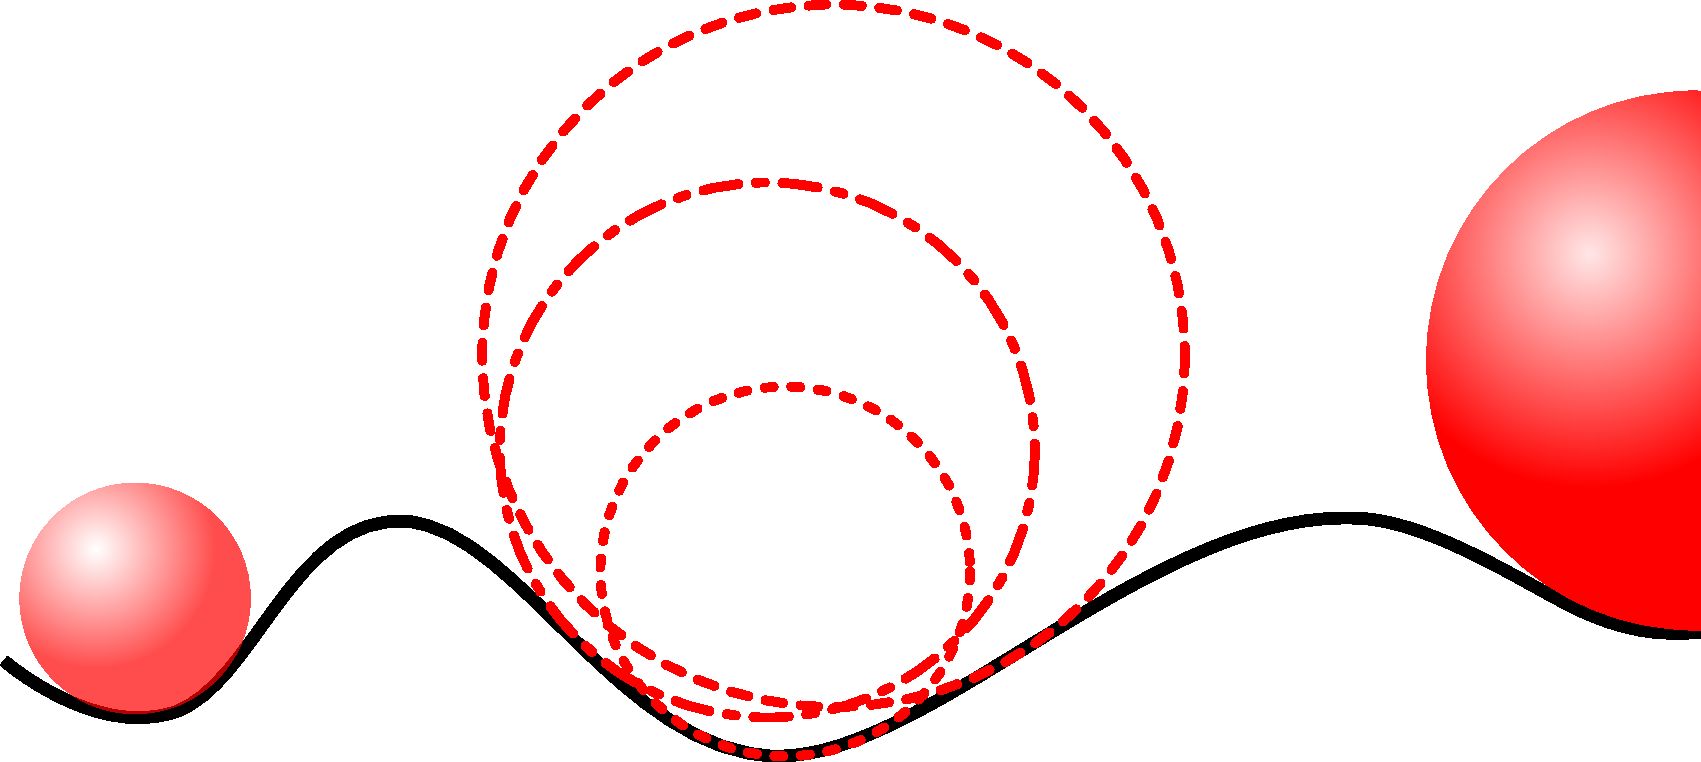
\includegraphics[width=0.88\linewidth,height=0.48\textheight,keepaspectratio]{../figs/pdf/en/fig-03-03.pdf}

% DOCX paragraph 237
\caption{\emph{The black line represents a one-dimensional cut of a generic curved
two-dimensional surface. The curvature}\index{curvature!radius} \emph{along the line varies
from point to point but can always be approximated locally with a circle (a
two-sphere}\index{two-sphere} \emph{in the two-dimensional surface). The radii of the
circles can vary and be very large if the line is almost straight.}}\label{fig:03-03}
\end{figure}

% DOCX paragraph 239
If, on the other hand, we wanted to consider spacetime in its four dimensions, we would
need to employ a four-dimensional sphere (which I am the first to admit is difficult to
imagine) osculating\index{osculating!sphere} at every point the local curvature of
four-dimensional spacetime.

% DOCX paragraph 240
Given these considerations, it will come as no surprise that a flat surface (which we
have seen is one with zero curvature) still has a radius of curvature associated with
it, but this radius is infinite. In the case of the Earth, the
curvature\index{curvature!radius (Earth)} radius is equal to its radius, which is about 6,400
kilometres, which is why it is necessary to go from the Caribbean to the North Pole to
measure the difference between the vectors. If we had conducted the experiment in a
square as large as the San Marco square in Venice, measuring a difference between the
vectors\index{vector} would have been much more difficult, although not impossible
with present technology.

% DOCX paragraph 241
The second consideration, triggered by the parallel transport\index{parallel transport} on a
two-sphere\index{two-sphere}, follows directly from the first and teaches us a
fundamental notion that we will use many times during this journey. Since our experience
of the physical world develops on length-scales of a few tens of kilometres (our view
does not go much further than that) and is built based on the gravitational field
present on Earth, it is almost inevitable to develop the perception\index{perception}
that the laws of physics are those of a flat spacetime, i.e., with zero curvature.
However, this is an incorrect impression, as much as it is to assume that the surface of
the Earth is flat only because it is difficult to appreciate its curvature. Fortunately,
Einstein's intuition was deep enough to break the constraints of our perception of flat
spacetime. We will return to this point in the following chapter.

% DOCX paragraph 242
The third consideration is that the mathematical tool employed so far (the parallel
transport of a vector along a closed circuit) is entirely general and can therefore also
be applied to surfaces whose curvature\index{curvature!complex} is much more complex than
those considered so far. When looking at Figure \ref{fig:03-04}, we can see a two-dimensional
surface whose curvature is different from point to point, except in the regions far from
the centre. In particular, if you think about the local radius of curvature, it is very
small near the origin and becomes larger as you move away from the centre. Exactly at
the origin, the radius of curvature is infinite because the function I have chosen in
representing the two-dimensional surface (that is, \emph{sin(r)/r} ) has a constant
value of about one near the origin. Finally, the example in Figure \ref{fig:03-04} shows that the
curvature\index{curvature! positive (convec)} can even change sign, becoming positive or negative
depending on whether the surface is \emph{convex}, as in the case of the
two-sphere\index{two-sphere}, or \emph{concave}\index{curvature!negative (concave)}.

% DOCX paragraph 243
\begin{figure}[htbp]
\centering
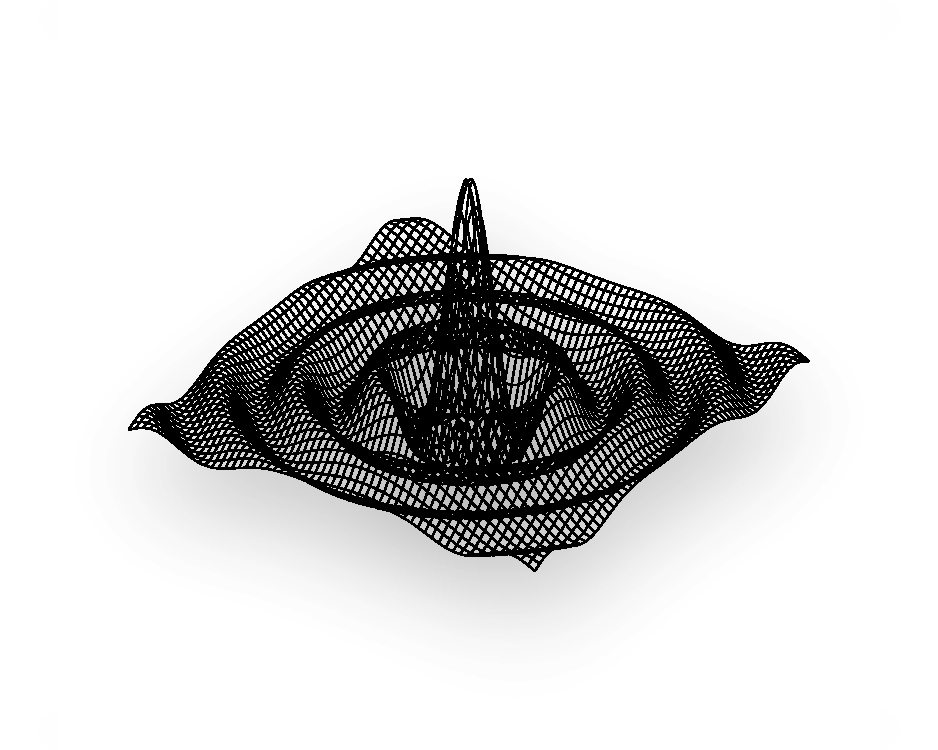
\includegraphics[width=0.88\linewidth,height=0.48\textheight,keepaspectratio]{../figs/pdf/en/fig-03-04.pdf}

% DOCX paragraph 244
\caption{\emph{A generic curved surface can be complex and have a local radius of
curvature that depends on the position, with a positive or negative value depending on
whether the surface is convex or concave.}}\label{fig:03-04}
\end{figure}

% DOCX paragraph 246
The theory of general relativity\index{general relativity} uses sophisticated mathematical
tools, many of them developed by mathematicians such as Tullio
Levi-Civita\index{Levi-Civita, Tullio} and Gregorio Ricci-Curbastro \index{Ricci-Burbastro, Gregorio} in the
early twentieth century, to measure the radius of curvature and its sign. Thanks to
them, it would not be difficult to develop apps, for instance, in our smartphones, which
would allow us to measure the local curvature of spacetime similar to those apps that
measure the local value of your altitude\index{spacetime!flat}\index{spacetime!curved}.

% DOCX paragraph 247
The examples given so far lead us to one final consideration: we have seen it is
possible to measure the level of curvature of a surface in two dimensions. The same can
be done for a surface in three dimensions (i.e., in a volume) and, by extension, in four
dimensions (such as in spacetime) or even in a surface of arbitrary dimensions. In other
words, it is possible to use the same logic and the same mathematical tools introduced
here in two dimensions to measure the \emph{curvature}\index{curvature|see{spacetime}} \emph{of
spacetime} and deduce whether it is flat or not.

% DOCX paragraph 250
\section{Curvature and The Einstein Equations}\label{sec:03-equations}

% DOCX paragraph 252
Now that we have seen what curvature is and which mathematical tools can be used to
measure it, we can take an important step forward and discover how the theory of general
relativity tightly links the presence of curvature to that of matter or
energy\index{energy}. This link is expressed by the Einstein equations proposed in
1915 and marked one of the most important chapters of modern physics. However, before
discussing these equations, it is necessary to recall another important equation (beware
the singular!), which is also related to Einstein but has nothing to do with gravity.
Indeed, it was introduced ten years before the theory of general relativity was proposed
and is part of the so-called theory of ``special
relativity''\index{special relativity}\index{relativity!special|see{special relativity}} (1905). This well-known equation
reads:

% DOCX paragraph 254
\begin{equation}\label{eq:03-02}
E = m\textcolor{gray}{c^{2}}
\end{equation}

% DOCX paragraph 256
This expression, also known as the \emph{Einstein equation}\index{Einstein!equation}, has
become an icon of the German physicist's scientific contribution. Although obtained
without having gravity in mind, it expresses an important idea that we will frequently
use in the rest of the book. In essence, through the = sign, Equation \eqref{eq:03-02} states the
equivalence between the
energy\index{energy!mass equivalence}\index{energy}\index{mass!energy equivalence} (\emph{E}, to the
left of the equal sign) and the mass (\emph{m}, to the right). The presence of the
square of the speed of light, \emph{c\textsuperscript{2}}, is essentially irrelevant to
what we are discussing here and serves only to make the two sides of the equation
comparable in terms of units (for this reason, it is shown in grey).\textsuperscript{\hyperlink{note:03-02}{2}}
In other words, Equation \eqref{eq:03-02} tells us that whenever we have a mass (it may be
represented by a feather or a boulder, an elementary particle, or a star), we also have
available a certain amount of energy.

% DOCX paragraph 257
This profound truth is behind the functioning of stars, which produce energy by fusing
(through the process of \emph{thermonuclear fusion}\index{thermonuclear fusion}) four hydrogen
atoms to form one of helium, whose mass is slightly smaller than the sum of the masses
of the four initial atoms of hydrogen. This small difference in mass is released in the
form of energy. The same principle applies to nuclear power plants where, through the
process of \emph{nuclear fission}, a complex atom such as uranium is ``broken down'' to
create many smaller ones, whose combined mass is less than the original. Again, the
difference in mass is released in the form of energy.

% DOCX paragraph 258
This is why, from now on, we will always talk about \emph{mass-energy}
\index{energy!mass equivalence}\index{mass!energy equivalence}without specifying whether it is a mass,
intended as a set of elementary particles (such as electrons, protons or neutrons) to
which we can associate a mass at rest or pure energy.

% DOCX paragraph 259
Now, without further preamble, we can move on to writing down the \emph{Einstein
equation}\index{Einstein!equations}\emph{s} (note the plural in this case!):

% DOCX paragraph 264
\begin{equation}\label{eq:03-03}
G_{\mu\upsilon} = \textcolor{gray}{\left( \frac{8\pi G}{c^{4}} \right)}T_{\mu\upsilon\ \ }
\end{equation}

% DOCX paragraph 266
It is easy to understand how, for the vast majority of you, these equations are as clear
as a Chinese text, that is, if you cannot read Chinese! Finding these equations
incomprehensible is perfectly normal --- you would need to attend a full university
course in general relativity\index{general relativity} to understand them. For example, for
the course I give in Frankfurt am Main in Germany, I need the best part of six months of
lectures and the introduction of a series of mathematical tools to be able to explain
and manipulate these equations in some detail.\textsuperscript{\hyperlink{note:03-03}{3}} However, in this
case, we can avoid being ``distracted'' by the mathematics and rather concentrate on the
deeper conceptual meaning of these equations, which represent the cornerstone of the
theory of general relativity and are, therefore, at the centre of Einstein's
revolutionary vision of gravity.

% DOCX paragraph 267
Let us start once again from the sign of equality in \eqref{eq:03-03}. It expresses an equivalence
between what appears on its left-hand side -- the \emph{Einstein tensor}
\index{tensor!Einstein} (\emph{G\textsubscript{µν}}) -- and its right-hand side. The latter
is made of two pieces: one in brackets, which has no physical meaning and for this
reason is shown in grey, and another tensor, namely the \emph{energy-momentum} tensor
(\emph{T\textsubscript{µν}}) \index{tensor!energy-momentum}. In essence, the Einstein equations
\eqref{eq:03-03} can also be read as the following conceptual equation:

% DOCX paragraph 270
\begin{equation}\label{eq:03-04}
(Einstein\ tensor) = (energy - momentum\ tensor)
\end{equation}

% DOCX paragraph 271
% Equation number is generated with the preceding equation.

% DOCX paragraph 273
Since the Einstein tensor represents a measure of the curvature of spacetime (in fact,
it is proportional to the Riemann tensor) while the energy-momentum tensor provides a
measure of the quantity of matter-energy present in spacetime (the greater the matter
and its concentration, the larger this tensor is), the complex equations \eqref{eq:03-03}
essentially state that:

% DOCX paragraph 276
\begin{equation}\label{eq:03-05}
(geometry\  - \ curvature) = (mass - energy)
\end{equation}

% DOCX paragraph 277
% Equation number is generated with the preceding equation.

% DOCX paragraph 279
This is arguably the most important concept in the whole book. It expresses exactly what
is contained in the Einstein equations \eqref{eq:03-03} in a more complex but also mathematically
elegant and physically revolutionary manner. In other words: \emph{wherever there is
matter (or energy)} \index{energy!mass equivalence}\index{mass!energy equivalence}\emph{, one can find a
spacetime curvature}. This is always true, no matter whether we are talking about the
mass of a galaxy or a grain of sand, a light ray, or a cannonball. Only the magnitude of
this curvature will vary, i.e., how pronounced it is. In the next chapter, we will learn
how to distinguish curvatures of different strengths and understand how nature is able
to produce them. First, however, we need to see how gravity enters into the conceptual
framework we have just discussed.

% DOCX paragraph 282
\section{Spacetime is an Elastic Fabric}\label{sec:03-fabric}

% DOCX paragraph 284
Although rich in important implications that we will explore in the rest of the book,
Equation \eqref{eq:03-05} still does not explain how gravity fits with what has been said so far.
In other words, it is probably not clear yet how the Einstein equations, summarised by
Equation \eqref{eq:03-05}, can explain what causes an apple to fall from a tree. This is the next
conceptual step we need to take and will require a little more concentration.

% DOCX paragraph 285
To understand how curvature and gravity are inextricably linked, let us start by
imagining a flat but elastic and deformable surface, for example, the sheet of a newly
made bed. In the absence of weights, it appears perfectly smooth and flat, and so it
remains until something disturbs its surface. This is shown in Figure \ref{fig:03-05}, which also
helps us to understand the meaning of the Einstein equations: the absence of
matter-energy leads to a spacetime with zero curvature, therefore flat. Within such
spacetime, we can take a vector\index{vector}, transport it in parallel along a
closed circuit and, at the end of the process, find that it is identical to the initial
one.

% DOCX paragraph 286
\begin{figure}[htbp]
\centering
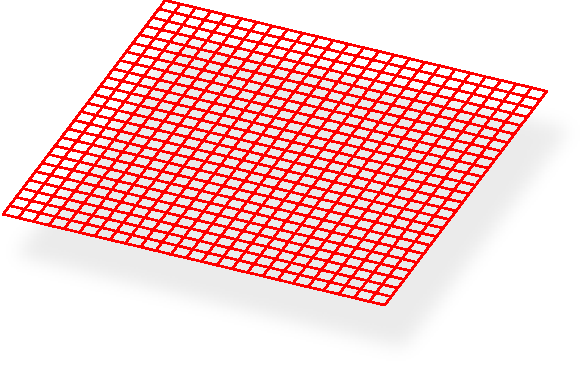
\includegraphics[width=0.88\linewidth,height=0.48\textheight,keepaspectratio]{../figs/pdf/en/fig-03-05.pdf}

% DOCX paragraph 287
\caption{\emph{The absence of matter-energy produces a spacetime without curvature and,
therefore, flat.}}\label{fig:03-05}
\end{figure}

% DOCX paragraph 288
To be picky, a spacetime of this type (strictly empty) cannot exist since the presence
of matter or energy, even if infinitesimal, would create a perturbation, hence removing
the absolute ``flatness''. However, the example is useful nonetheless because it is
often possible to consider a ``nearly flat'' or ``locally flat'' spacetime that, though
not flat on large scales, is flat in a small region. \index{spacetime!flat}

% DOCX paragraph 289
Let us now try to imagine what would happen if we placed a heavy object on that sheet,
such as a bowling ball. As you can easily guess, it would ``curve'' around the weight,
exactly as shown in Figure \ref{fig:03-06}. This example offers us a useful analogy with what is
expressed by the Einstein equations: the presence of matter (or energy)
\index{energy!mass equivalence}\index{mass!energy equivalence}produces a spacetime with non-zero curvature and
is, therefore, curved\index{spacetime!curved}. If we took a vector and transported it in
parallel along a closed circuit inside it, at the end of the path we would find it is
different from the initial one.\textsuperscript{\hyperlink{note:03-04}{4}}

% DOCX paragraph 291
\begin{figure}[htbp]
\centering
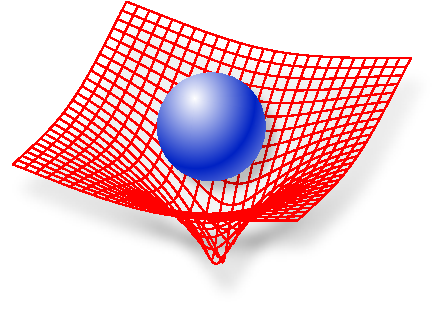
\includegraphics[width=0.88\linewidth,height=0.48\textheight,keepaspectratio]{../figs/pdf/en/fig-03-06.pdf}
\caption{\emph{The presence of matter-energy (represented here by a sphere, which could
be a planet or a grain of sand) produces a spacetime with non-zero curvature and is,
therefore, curved.}}\label{fig:03-06}
\end{figure}

% DOCX paragraph 292
The example of the sheet gives us the opportunity for three observations. The first has
to do with an essential aspect of Figure \ref{fig:03-06} that should not be missed: the curvature
produced by the bowling ball is not identical everywhere but varies from point to point.
In particular, it is very small at the edges of the sheet, which will appear almost
flat, and more pronounced as it approaches the point where the object is placed, where
it will be at its maximum size. In other words, it is natural to expect that, under
generic conditions, curvature is a function of position; only in exceptional
circumstances (as in the case of a two-sphere\index{two-sphere}) is the curvature
constant.

% DOCX paragraph 293
The second consideration concerns the ``shape'' of the deformation. Although it may seem
obvious that the presence of the bowling ball produces a \emph{concave} or
\emph{positive} curvature, the Einstein equations reveal that it is also possible to
have, in a completely equivalent manner, a \emph{convex} or \emph{negative} curvature.
Our experience is that the matter around us, and with which we normally conduct
experiments, actually produces a positive curvature, precisely as illustrated in Figure
\ref{fig:03-06}. However, it does not exclude --- indeed, the Einstein equations allow for it ---
the existence of matter that produces a \emph{negative} curvature.

% DOCX paragraph 294
The third and final observation has to do with the impact of the curvature. It is
important to appreciate that the presence of a curvature will affect the dynamics (i.e.,
the motion) of any object around it. For example, let us imagine adding another smaller
and lighter sphere next to the bowling ball, such that it does not produce a curvature
of the sheet comparable to the first. In such a scenario, and, in the absence of
friction, the second object will be forced to move, ``falling'' towards the centre of
the curvature produced by the bowling ball. With this example, we can therefore
understand how gravity manifests itself in geometric terms. By modifying the spacetime
in which motion occurs, curvature produces a variation in the dynamics of the bodies,
which would otherwise remain in the state of rectilinear motion or rest.

% DOCX paragraph 297
\section{Curvature and Gravity}\label{sec:03-gravity}

% DOCX paragraph 299
Having introduced and discussed the concepts of spacetime and curvature, we are finally
ready to return to the simple but obscure statement \eqref{eq:03-01}. I recall that it read:

% DOCX paragraph 300
\[\begin{pmatrix}
gravity\ is\ the\ manifestation\ of\  \\
spacetime\ curvature
\end{pmatrix}\]

% DOCX paragraph 302
At this point in my course of general relativity, the bewildered and sceptical looks
that appear on the students' faces when they first encounter this statement are replaced
by subtle smiles of satisfaction. The expression of someone on realising that: ``Of
course! How could it be otherwise?''. Not only is the sentence no longer cryptic, but it
has also become deeply fascinating.

% DOCX paragraph 303
In other words, Einstein has stated that if spacetime is empty, in the sense that it is
devoid of any matter producing a curvature, then it is also flat. In this case, every
object in it will maintain its state of motion: depending on its initial condition, it
will continue to be stationary or move with a constant speed along a straight line (this
is indeed the principle of inertia). However, if spacetime contains
matter-energy\index{energy!mass equivalence}\index{mass!energy equivalence}producing a curvature, then every
object in it will be affected by this curvature through a modification of its state of
motion. Thus, those objects initially at rest will no longer be able to remain so. On
the other hand, those objects moving at a constant speed along a straight line will see
their trajectory and speed change.

% DOCX paragraph 304
It follows that, in this different and decidedly revolutionary view of gravity, if the
apple\index{apple (falling)} falls from a tree, it is not because there is a gravitational
force\index{gravitational!force} that draws it towards the Earth. What happens is that the
Earth, with its content of matter and energy, curves spacetime around itself and forces
objects to move accordingly. When the apple is no longer attached to the tree, which
until then prevented it from moving freely, it can only move following the local
curvature of spacetime and therefore towards the centre of the Earth. And that is
actually what it does! Well, at least until it encounters the planet's surface, which
prevents it from continuing further. This is what Figure \ref{fig:03-07} shows in a very schematic
(and obviously out of scale!) manner.

% DOCX paragraph 306
\begin{figure}[htbp]
\centering
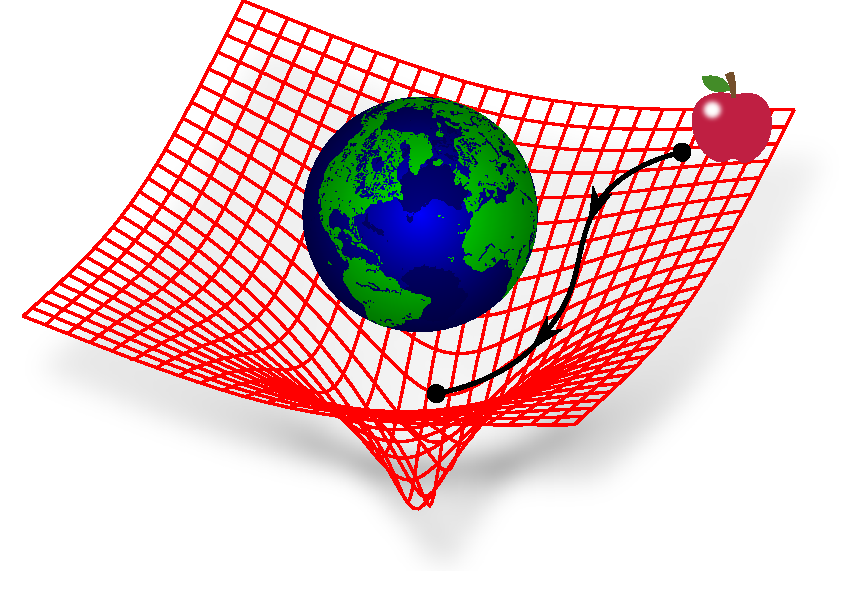
\includegraphics[width=0.88\linewidth,height=0.48\textheight,keepaspectratio]{../figs/pdf/en/fig-03-07.pdf}
\caption{\emph{Interpretation of the fall of an apple in Einstein's theory of
gravitation: the Earth produces a curvature of spacetime, and the apple must move
following it, thus ``falling'' towards the centre of the planet.}}\label{fig:03-07}
\end{figure}

% DOCX paragraph 307
An additional comment could be added here, which I am sure you will understand perfectly
at this point. The reason, once free from the tree, the apple does not move away into
interplanetary space is linked to the \emph{sign} of the curvature, that is, to the fact
that the Earth produces a positive (or concave) curvature. However, if we hypothetically
admitted the existence of a type of matter producing a negative curvature, then the
surface of the ``sheet'' in Figure \ref{fig:03-06} would be deformed with a convex curvature, and
gravity would behave in the opposite manner: it would be not attractive but
\emph{repulsive,} with the apple flying into space! Fortunately, even in the presence of
this ``change of sign'', the title of this book would remain valid. Indeed, in this
case, gravity would be even more attractive to our attention!

% DOCX paragraph 308
The example just suggested of a repulsive gravity may seem absurd at first sight, but it
is exactly what we think is happening right now to the universe as a whole. By observing
very distant supernova\index{supernova} explosions, it is possible to deduce that the
universe is currently in a phase of accelerated expansion. The cause of this phenomenon
is not yet clear, but it could be linked to \emph{dark
energy}\index{energy!dark }\index{dark energy}: a tenuous form of energy that would
generate a negative curvature. As a result, at least on a cosmic scale, it would appear
to produce an action similar to that of \emph{antigravity}\index{antigravity}!

% DOCX paragraph 311
\section{Nothing Moves on a Straight Line}\label{sec:03-geodesics}

% DOCX paragraph 313
We have already discussed in note 4 how the example proposed in Figure \ref{fig:03-06} contains a
logical flaw. There, to explain curvature and gravity, we have used a bowling ball
already immersed in a gravitational field (the terrestrial one) so that it curves the
sheet precisely because it is already in such a field. Therefore, we are using the
dynamics of an object in a gravitational field to explain what curvature is, which we
can then say is the very origin of gravity. The circularity of the argument is evident.
Fortunately, however, this circularity is also harmless: it just shows us that the
curved-sheet analogy is very valuable but not perfect.

% DOCX paragraph 314
Indeed, a better analogy can be used to visualise and measure the curvature without the
aid of sheets and bowling balls. However, I still need a bit of your attention to do
this but rest assured that it will be worth it as we will discover one of the most
useful tools in modern astronomy.

% DOCX paragraph 315
Let us go back to the idea of an empty and, therefore, flat spacetime where an object
follows the principle of inertia: it remains stationary if initially stationary, or it
continues in its uniform rectilinear motion (i.e., at constant speed). However, it is
clear that this can no longer be true if the spacetime is curved. In this case, in fact,
the trajectory of the object will be modified by the curvature and will have to adapt
accordingly. Hence, uniform rectilinear motion can no longer exist in a curved
spacetime, where instead, every motion must necessarily be curved. In other words,
nothing moves in a straight line in a spacetime containing matter-energy, except for
infinitesimally short distances.

% DOCX paragraph 316
The conclusion just reached has two interesting consequences. The first is related to
the common experience that a straight line represents the minimum distance between two
points, the so-called \emph{geodesic}\index{geodesic} between them. This is
obviously true in flat spacetime but ceases to be true in a curved spacetime, where a
straight line no longer represents the minimum distance.

% DOCX paragraph 317
This consideration is less bizarre than it might appear, and two concrete examples will
help us understand how it is quite obvious. First, suppose you are moving along a curved
surface and need to go from point A to point B, as shown in Figure \ref{fig:03-08}.

% DOCX paragraph 318
\begin{figure}[htbp]
\centering
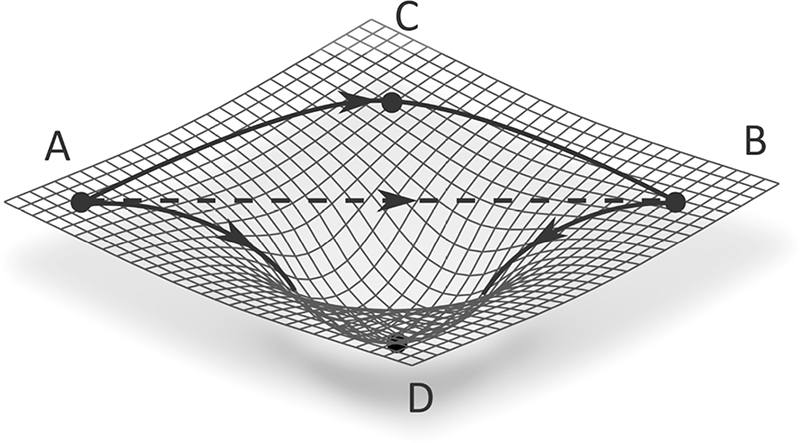
\includegraphics[width=0.88\linewidth,height=0.48\textheight,keepaspectratio]{../figs/source/en/fig-03-08.png}

% DOCX paragraph 320
\caption{\emph{In a curved spacetime, a straight line is not the shortest path to
connect two points (i.e., a geodesic}\index{geodesic}\emph{). In the figure, the ACB
trip is the geodesic between A and B.}}\label{fig:03-08}
\end{figure}

% DOCX paragraph 322
You may find yourself in a similar situation when walking on the hills near Trieste in
Italy, where these types of deformations of the terrain are very common. Obviously, you
would not be able to reach B from A in a straight line (well, unless you fly, but we
will consider this case in the next example), and instead, you would be forced to follow
the surface of the terrain through the route ACB or ADB, choosing the shortest and least
tiring one. To clarify, let us suppose it is the first one (although, in different
conditions, it could be the second). In this case, the route ACB represents the
\emph{geodesic}\index{geodesic} between A and B, the curve that when travelled
measures the shortest distance between the two points A and B.\textsuperscript{\hyperlink{note:03-05}{5}}

% DOCX paragraph 323
For the second example, just think of the routes that aeroplanes or ships follow to move
from one point to another on our planet. These routes also represent geodesics since
they are calculated to minimise fuel costs and, therefore, trace the shortest distance
between the two points. However, since planes and ships are still forced to move along
the Earth's curved surface, these geodesics cannot be straight lines: they must
necessarily be curves, i.e., the geodesics of a curved spacetime. This has an important
implication: we have seen that it is possible to approximate locally a curved spacetime
with a flat spacetime; by the same principle, aeroplanes and ships will seem to move
along trajectories that appear as straight lines on small length-scales, but that are
actually curved on scales comparable to the radius of Earth's curvature.

% DOCX paragraph 324
The second important consequence of the conclusion that nothing moves in a straight line
is indeed linked to astronomy. Observations tell us that the universe is fundamentally
\emph{empty}, with the exception of local concentrations of matter, which manifest
themselves in the form of planets, stars, galaxies, clusters of galaxies, and so on.
Thus, in the spacetime describing our universe, vast regions (representing the majority
of the spatial volume) are \emph{nearly flat}. \index{spacetime!flat (nearly)} In these regions,
objects with a mass move along straight lines that remain parallel if initially
parallel. However, in those regions where matter is present, which are much rarer and
represent a small fraction of the volume, the spacetime is instead curved, and the
trajectory of objects with a mass cannot be rectilinear: two paths that start as
parallel must necessarily diverge or converge.

% DOCX paragraph 325
Based on these considerations, we can ``easily'' create tools that allow us to verify
whether spacetime is, in fact, flat or curved, even without resorting to the aid of
sheets and bowling balls. It would be ``enough'' to take small objects with mass, such
as microsatellites, and launch them towards a fairly distant celestial body, such as
Proxima Centauri\index{Proxima Centauri} (which is the closest star to us after the Sun and
is only 4.24 light years away), taking care that their trajectories are initially
parallel. At this point, it would be sufficient to check the separation between the
objects when they have reached their destination, in our case after about 270,000 years
(assuming that they are moving at the maximum speed reached so far by an artificial
satellite). Depending on whether the separation has decreased or increased compared to
the initial one, we will know whether they will have encountered regions of spacetime
with positive or negative curvature during the journey.

% DOCX paragraph 326
This example is wildly unrealistic, and although conceptually correct, it is impossible
in practice; it is only the abstruse idea of a theoretical physicist. However, a hundred
years ago, Einstein suggested an experiment that is quite similar conceptually and was
also physically feasible for the technology of those times. Indeed, through that
experiment he convinced even the most sceptical scientists of the time about the
correctness of his bizarre theory of gravitation.

% DOCX paragraph 327
To better understand what Einstein proposed, we need to go back to his equation on the
equivalence between mass and energy, that is, Equation \eqref{eq:03-02}. That equation allows us to
deduce that, if in a curved spacetime the motion of an object \emph{with a mass} is not
rectilinear, then the same must apply to the motion of an object \emph{without a mass},
for example, a light ray, which we also refer to as a photon\index{photon}. In
other words, a light ray propagating in a curved spacetime will be forced to follow a
curved trajectory. At the risk of being pedantic, but with the intent of being extra
precise, I should remark that a light ray always moves along a
geodesic\index{geodesic}, a line of minimal separation. This will be a straight line
only in a flat spacetime and will instead be a curved line in more general conditions,
like those in a curved spacetime.

% DOCX paragraph 328
When compared to satellites, photons offer two additional advantages: they are much
faster than any object with mass (indeed, they travel at the maximum speed allowed), and
they are emitted in abundance by celestial bodies such as Proxima
Centauri\index{Proxima Centauri}. Therefore, all we have to do is use telescopes to
intercept these photons and deduce whether their trajectory has been modified or not by
the presence of curvature.

% DOCX paragraph 329
This is exactly what Einstein proposed about a hundred years ago with the famous 1919
total solar eclipse experiment, the basic idea of which is shown in Figure \ref{fig:03-09}. In
essence, Einstein made a very clever consideration: if a ray of light is deflected by
the presence of a massive object (for example, the
Sun\index{Sun!eclipse (see solar)}\index{solar eclipse}) which curves spacetime and tends to
``attract'' it, then it is in principle possible to ``see'' what lies behind that
object!

% DOCX paragraph 330
Obviously, the ability to deflect a light ray depends on the strength of the curvature
produced by the celestial body and therefore (as we will see in the next chapter), on
its mass and radius. Doing some math with an approximate version of his equations,
Einstein concluded that while not possible to observe objects placed \emph{exactly}
behind the Sun, the curvature generated by our star would be sufficient to show us
objects placed close to its projected surface.

% DOCX paragraph 331
At that point, there was only one problem to solve: the Sun is the dominant source of
light around us, and it is therefore impossible to identify the small contribution to
the brightness made by a star near its edge. To check this idea, we would need to turn
off the Sun! Fortunately for us, this cannot be done, but it is what essentially happens
during a total eclipse. In that case, the light reaching us from the Sun is practically
suppressed, so that celestial objects close to its projected surface could be seen ---
well, at least according to general relativity\index{general relativity}! The experiment
suggested by Einstein, therefore, consisted of observing a total solar
eclipse\index{solar eclipse} from an optimal position and determining which of the stars
close to its edge, and theoretically invisible because covered by the Sun, were actually
visible.

% DOCX paragraph 334
\begin{figure}[htbp]
\centering
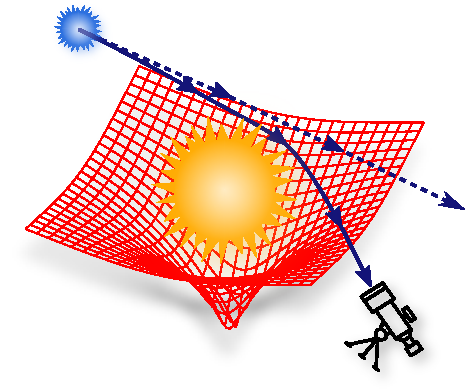
\includegraphics[width=0.88\linewidth,height=0.48\textheight,keepaspectratio]{../figs/pdf/en/fig-03-09.pdf}

% DOCX paragraph 335
\caption{\emph{One of Einstein's most important predictions is that light cannot travel
in a straight line in a curved spacetime. As a result, it is possible to observe
celestial bodies even when they are hidden by other objects in the foreground.}}\label{fig:03-09}
\end{figure}

% DOCX paragraph 336
I am omitting here the historical details of the adventurous expedition led by the
English astronomer Sir Arthur Eddington\index{Eddington, Sir Arthur}, a great admirer of Einstein
and one of the few initial supporters of the theory of general relativity. Observations
made by Eddington\index{Eddington, Sir Arthur} on May 29, 1919, on Príncipe Island, at that time
a Portuguese territory but now part of the Democratic Republic of São Tomé e Príncipe
(an Atlantic archipelago located in the Gulf of Guinea), revealed that it was indeed
possible to measure a deflection of light produced by distant stars and that this was
equal to about 1.75 arcseconds. The measurement of a physical phenomenon impossible in
Newtonian gravity, but that coincided with what had been predicted by the revolutionary
theory of general relativity\index{general relativity}, represented the final straw for
Newton's theory and the scientific consecration of all the ``bizarre'' ideas that we
have discussed in this chapter: spacetime, energy, matter, curvature ... Clearly, these
ideas were not bizarre at all!

% DOCX paragraph 337
The phenomenon just described (namely, that light cannot propagate in a straight line in
a curved spacetime) is one of the most useful applications of the theory of the
brilliant German physicist, so much so that it has been jokingly renamed ``the gift of
Einstein to astronomy''. The reason behind this statement is easy to understand. Just
like the Sun, in fact, any astronomical object can act as a \emph{gravitational lens,}
deflecting the light coming from other objects and not only distorting their appearance
but also amplifying it, thus making visible those objects whose image would otherwise be
too weak. This is exactly what a lens does: it concentrates a beam of parallel light
rays in one point --- its focus.

% DOCX paragraph 338
Exploiting these interesting deflection effects, astronomers can now obtain multiple and
amplified images of galaxies at huge distances from us, in what is normally referred to
as \emph{gravitational}\index{gravitational!lensing} \emph{lensing}\index{lensing|see{gravitational}}.

% DOCX paragraph 339
As a final comment, I note that this phenomenon can also occur when the object acting as
a lens is not visible because it does not emit light, although it is quite massive. In
this case, the presence of the ``lensing object'' can be deduced from the curvature of
spacetime that it induces, and which manifests itself through the distortion of images
of other distant objects. A classic example of this type of lensing is that produced by
so-called \emph{dark matter}\index{dark matter}, which does not emit light. Instead,
its presence is detectable through the gravitational action it produces on a galactic
scale by affecting the speed at which stars in spiral galaxies rotate around the centre
and revealing that it is present in the form of a huge spherical halo.

% DOCX paragraph 358
\begin{figure}[htbp]
\centering
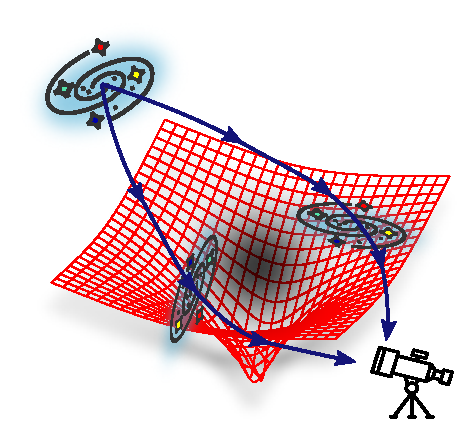
\includegraphics[width=0.88\linewidth,height=0.48\textheight,keepaspectratio]{../figs/pdf/en/fig-03-10.pdf}
\caption{\emph{Compact astronomical objects can act as gravitational lenses and
concentrate emissions from distant sources or produce multiple images. Gravitational
lenses can also be invisible, as is the case with dark
matter}\index{dark matter}\emph{.}}\label{fig:03-10}
\end{figure}

% DOCX paragraph 360
Figure \ref{fig:03-10} illustrates schematically how the presence of invisible dark
matter\index{dark matter} still produces a curvature of local spacetime, which
generates multiple and distorted images of distant galaxies. In this case, by analysing
how images of celestial objects are distorted, observations can be used to study the
properties of dark matter, such as its mass and distribution.

% DOCX paragraph 361
But it does not end here! In Chapter 7, we will see how the deviation of a beam of light
in the vicinity of a strongly curved spacetime gives rise to bizarre phenomena such as
double and triple images, amplifications, and absorptions. In the same chapter, I will
also explain how it is possible to produce the image of a black hole, as done recently
by my research group in collaboration with the Event Horizon Telescope.
